%PIP-412029OA046
\documentclass[rc,ec]{physicsinprogress}

\pipvolume{2}
\pipissuedate{Feb. 2026}

\usepackage{siunitx}

\begin{document}


\title{Determining the interplanar spacing of graphite using electron diffraction}% Force line breaks with \\


\author{Sema'Je Zechariah Farmer}
\affiliation{%
Department of Physics and Astronomy,  Carthage College, 2001 Alford Park Drive, Kenosha, WI 53140, USA
}%
\pipdates{January 29, 2026}{February 5, 2026}


%\date{\today}% It is always \today, today,
             %  but any date may be explicitly specified

\begin{abstract}

When firing a beam of electrons at a crystal lattice, those electrons will diffract. The pattern that forms as a result of that diffraction will depend on and be unique to the crystal structure of the targeted lattice. By combining de Broglie's theory with Bragg's law, a relationship can be derived between the diffraction angle of electrons and their accelerating voltage. This relationship can then be used to determine fundamental structural information about the crystal. Using this method, the inter-planar Spacing for $d_{100}$ and $d_{110}$ of graphite were determined to be  $1.7 \pm 0.1 \text{ Å}$ and $1.4\pm 0.2 \text{ Å}$ respectively.

\end{abstract}

%\keywords{Suggested keywords}%Use showkeys class option if keyword
                              %display desired
\maketitle

%\tableofcontents

\section{\label{sec:level1} Introduction}
In the 18th century, Thomas Young conducted his infamous double slit experiment, challenging Newton's particle theory by proving the wave-like properties of light \cite{Young1802}. Later in the 19th century, Einstein published his work interpreting Philipp Lenard's experimental results on the photoelectric effect. In this work, Einstein concluded that light consists of quanta called photons, which act as particles \cite{Arons1965}. This introduced the idea of wave-particle duality, the notion that these photons may behave as waves or particles depending on the situation. Building on Einstein's work, Louis de Broglie hypothesized that wave-particle duality may also hold for physical objects, not just for light \cite{Broglie1924}.

In modern times, multiple experiments have shown the wave-like behavior of particles, but the first to prove de Broglie's hypothesis were electron diffraction experiments such as the Davisson-Germer experiment. The original intent of this experiment was to continue studying the angular distribution of electrons scattered by a nickel target. While collecting data, an accident occurred, requiring the target to be cleaned. After cleaning the target with high heat and effectively recrystallizing it, a possible relationship between scattering intensity and crystal direction was found, prompting further investigation. During this new investigation, they observed intensity peaks at specific angles, very similar to interference patterns and characteristic of wave-like behavior \cite{Davisson1927}. This was the first confirmation of de Broglie's theory. From there, known values of the target's interplanar spacing and diffraction angles were used to estimate the wavelength using Bragg's law. Those wavelength values were then compared to values calculated from de Broglie's formula. The results of that comparison were similar: calculations using both de Broglie's formula and Bragg's law yielded the same wavelength values. These results solidified de Broglie's theory and the idea of wave-particle duality for all matter.





\section{Theory}



This experiment uses a very similar setup to the Davisson-Germer experiment and the same basic principles to work towards a slightly different goal. Instead of using measurements to estimate and verify wavelength calculations, this experiment aims to estimate the values of $d_{100}$ and $d_{110}$ for graphite. The Davisson-Germer experiment confirmed that de Broglie's formula can be used to accurately calculate the wavelength of an electron beam \cite{Broglie1924}. With this alternate method for determining wavelength and the ability to measure deflection angles, Bragg's law can be used to estimate $d$. Starting with de Broglie's formula


\begin{equation}
\lambda = \frac{h}{p},
\label{dbwl}
\end{equation}

where $h$ is Planck's constant and $p$ is the momentum of the electrons as they are accelerated through a potential difference. This potential difference determines the speed that the electrons will travel at, and by translation, their momentum \cite{Davisson1927}. Bragg's condition states that

\begin{equation}
\ 2d\sin \theta = \lambda n ,
\label{bragg}
\end{equation}
where $d$ is the inter-planar spacing and $\lambda$ is the wavelength, and $\theta$ is the angle between the target lattice and the incident beam, and $n$ is the order of reflection\cite{Bragg1922}. In experiments like this one, it is common to simplify by assuming $n=1$. This is because in electron diffraction, first-order reflections tend to be much more intense and visible than the higher-order ones \cite{MEYER2021}. If data is collected on the most visible reflections, then it likely corresponds to first-order reflections. 

\begin{figure}
    \centering
    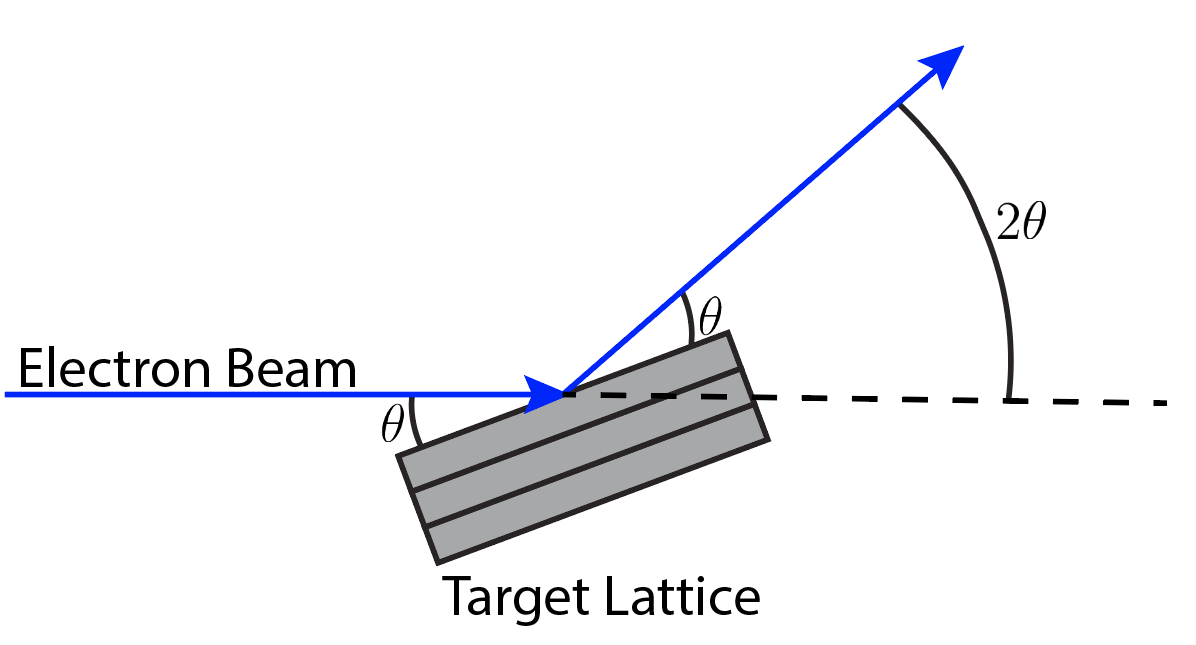
\includegraphics[width=0.9\linewidth]{2Theta.png}
    \caption{Diagram for showing deflection angle for a beam of electrons bouncing off a target lattice.}
    \label{fig:2sintheta}
\end{figure}

To better understand where $\theta$ comes from, refer to fig \ref{fig:2sintheta} above. The diagram shows an electron beam approaching the lattice at an angle $\theta$ with respect to the lattice. Then it deflects off the lattice with the same relative angle. For the beam to approach and depart at an angle $\theta$ relative to the lattice, it must have deflected by a total of $2\theta$ relative to the horizontal. This distinction becomes especially important when combining de Broglie's formula with Bragg's law to get

\begin{equation}
\sin\theta = \frac{h}{2d \sqrt{2m_e}}E^{-\frac{1}{2}},
\label{combin}
\end{equation}
\\

Where $E$ is the energy of the diffracted beam given by $E=qV$. Equation \ref{combin} shows a linear relationship between $\sin\theta$ and $E^{-1/2}$. So if de Broglie was indeed correct about particles demonstrating wave-like behaviors, then a plot of measured values for $\sin\theta$ against the measured values for $V^{-1/2}$ should be linear just as the math suggests.

To test this and obtain real, measured values, an apparatus similar to the diagram shown in Fig. \ref{fig:Bulb} is used. In this diagram, a beam of electrons is emitted from the filament, energized to the order of keV, and sent into the target lattice where it diffracts.

\begin{figure}
    \centering
    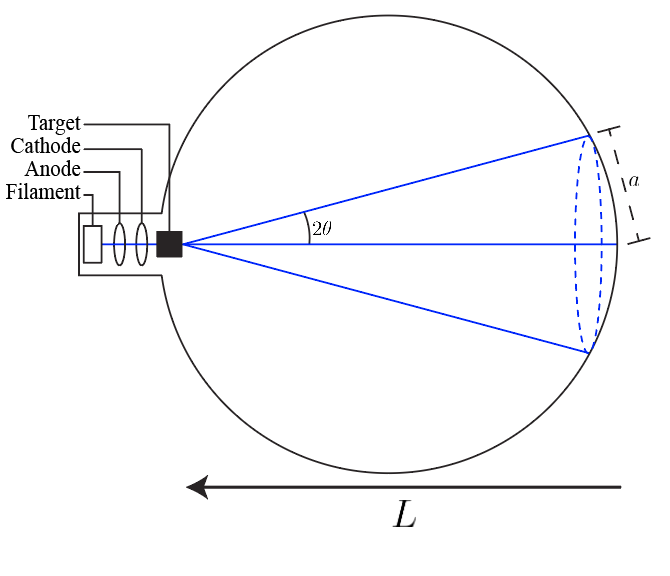
\includegraphics[width=\linewidth, angle=0]{Bulb new.png}
    \caption{A schematic representation of the diffraction tube on the 3B Scientific UE501050 electron diffraction apparatus.}
    \label{fig:Bulb}
\end{figure}
As seen in Fig. \ref{fig:Bulb}, the diffraction pattern forms a ring on the surface of the bulb. By measuring the distance $a$ from the center of the ring to the ring itself, a value for $\sin\theta$ can be obtained. 

\begin{equation}
    \sin2\theta=\frac{a}{L}.
    \label{2theta}
\end{equation}

Fig. \ref{fig:Geo} provides a more in-depth look at the geometry involved in obtaining Eq. \ref{2theta}. 


\begin{figure}
    \centering
    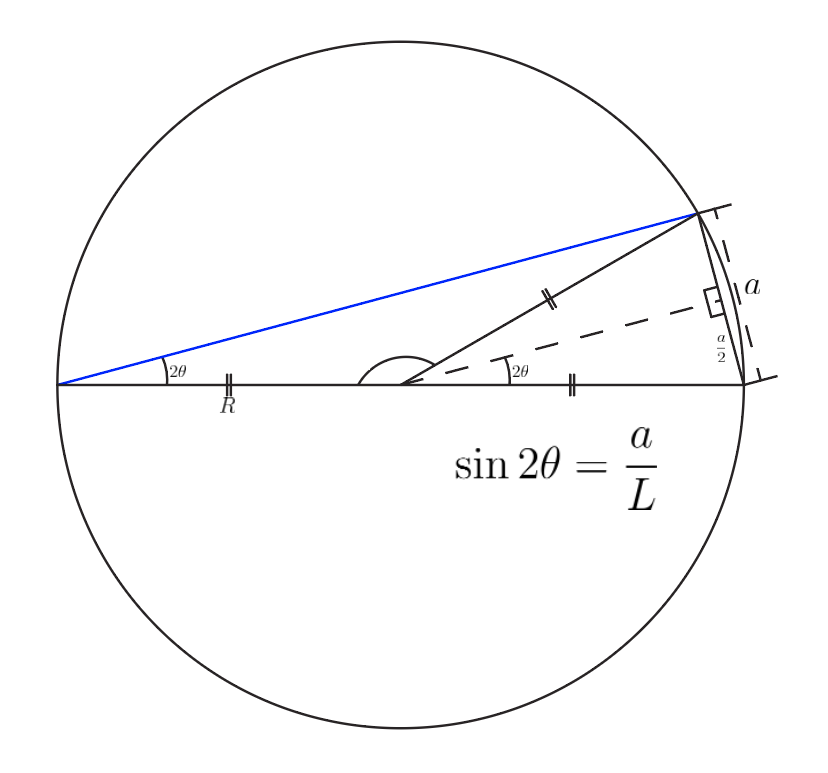
\includegraphics[width=3in, angle=0]{Geo new.png}
    \caption{A look at the geometry behind determining $\sin\theta$.}
    \label{fig:Geo}
\end{figure}


$L$ is the distance from the crystal lattice to the screen on the opposite end of the bulb. $L/2$ is roughly the radius of the bulb. The measured side length $a$ completes an isosceles triangle. Equation \ref{2theta} was derived by using the trigonometric ratio for $\sin$ on one of the two right triangles formed by an isosceles triangle. Given the trig identity $\sin 2\theta = 2\sin\theta \cos\theta$ and the fact that for small angles $\cos\theta\approx1$, Eq. \ref{2theta} simplifies to

\begin{equation}
    \sin\theta=\frac{a}{2L},
    \label{sintheta}
\end{equation}

This equation provides a way to calculate values of $\sin\theta$ from the measured value of $a$ and the $L$ value provided in the manual. With that, all that remained was to take the physical measurements. 

For data collection, voltage was varied between 3 and 4.5 kV. In this range, two rings formed on the bulb. These rings formed because the target lattice is a thin film consisting of graphite powder. The powder contains many small graphite crystals, so diffraction occurs at various orientations, resulting in ring formation. Measurements of $a$ were taken for each ring at multiple points across the voltage range. The rings, while bright, were not sharp, so the measurements of $a$ have an estimated uncertainty of $3$ mm to account for the fuzziness of the rings. The other value, $L$, was not measured during the experiment but was given in the device manual. That value has an estimated uncertainty of $ 2$ mm. 

\begin{figure}
    \centering
    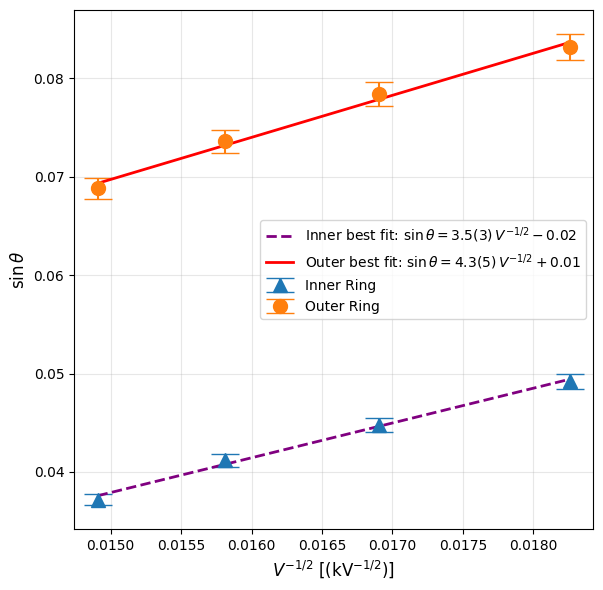
\includegraphics[width=3in, angle=0]{Plot New.png}
    \caption{Linear regression plot of $\sin\theta$ Vs. $V^{-1/2}$}.
    \label{fig:Plot}
\end{figure}

Fig. \ref{fig:Plot} is the plot resulting from the measurements of $a$ taken from each ring at four different beam energies. For both rings $\sin\theta$ increases as $V^{-1/2}$ increases. This trend is consistent with the linear relationship $\sin\theta \propto E^{-1/2}$ shown by Eq. \ref{combin}. The fact that the experimental results remain consistent with the earlier mathematical predictions confirms the accuracy of de Broglie's formula for this experiment. 


From here, the data can be used to calculate the $d_{100}$ and $d_{110}$ values of the crystal lattice using the slopes of the lines denoted by $S$. Solving Eq. \ref{combin} for d and substituting slope $S$ in place of $\sqrt V \sin\theta$ yields the equation 

\begin{equation}
    \ d = \frac{h}{2m\sqrt{2S_eq}}.
    \label{latpar}
\end{equation}

Plugging the slopes of the best-fit lines for each ring's measurements into equation \ref{latpar}
yielded an inner ring value of $1.7 \pm 0.1 \text{Å} $ and an outer ring value of $1.4\pm 0.2\text{Å}$. With two values for d, the next step is to figure out which value corresponds to which interplanar spacing. The answer becomes mathematically evident when combining Eqs. (3,5).  

\begin{equation}
    \frac{a}{2L} = \frac{h}{2d \sqrt{2m_e}}E^{-\frac{1}{2}}.
    \label{proof}
\end{equation}
The resulting equation shows $a$ to be inversely proportional to $d$, implying that ring projections with larger radii correspond to smaller interplanar spacings. A similar result is observed in the crystal structure of graphite itself.

\begin{figure}
    \centering
    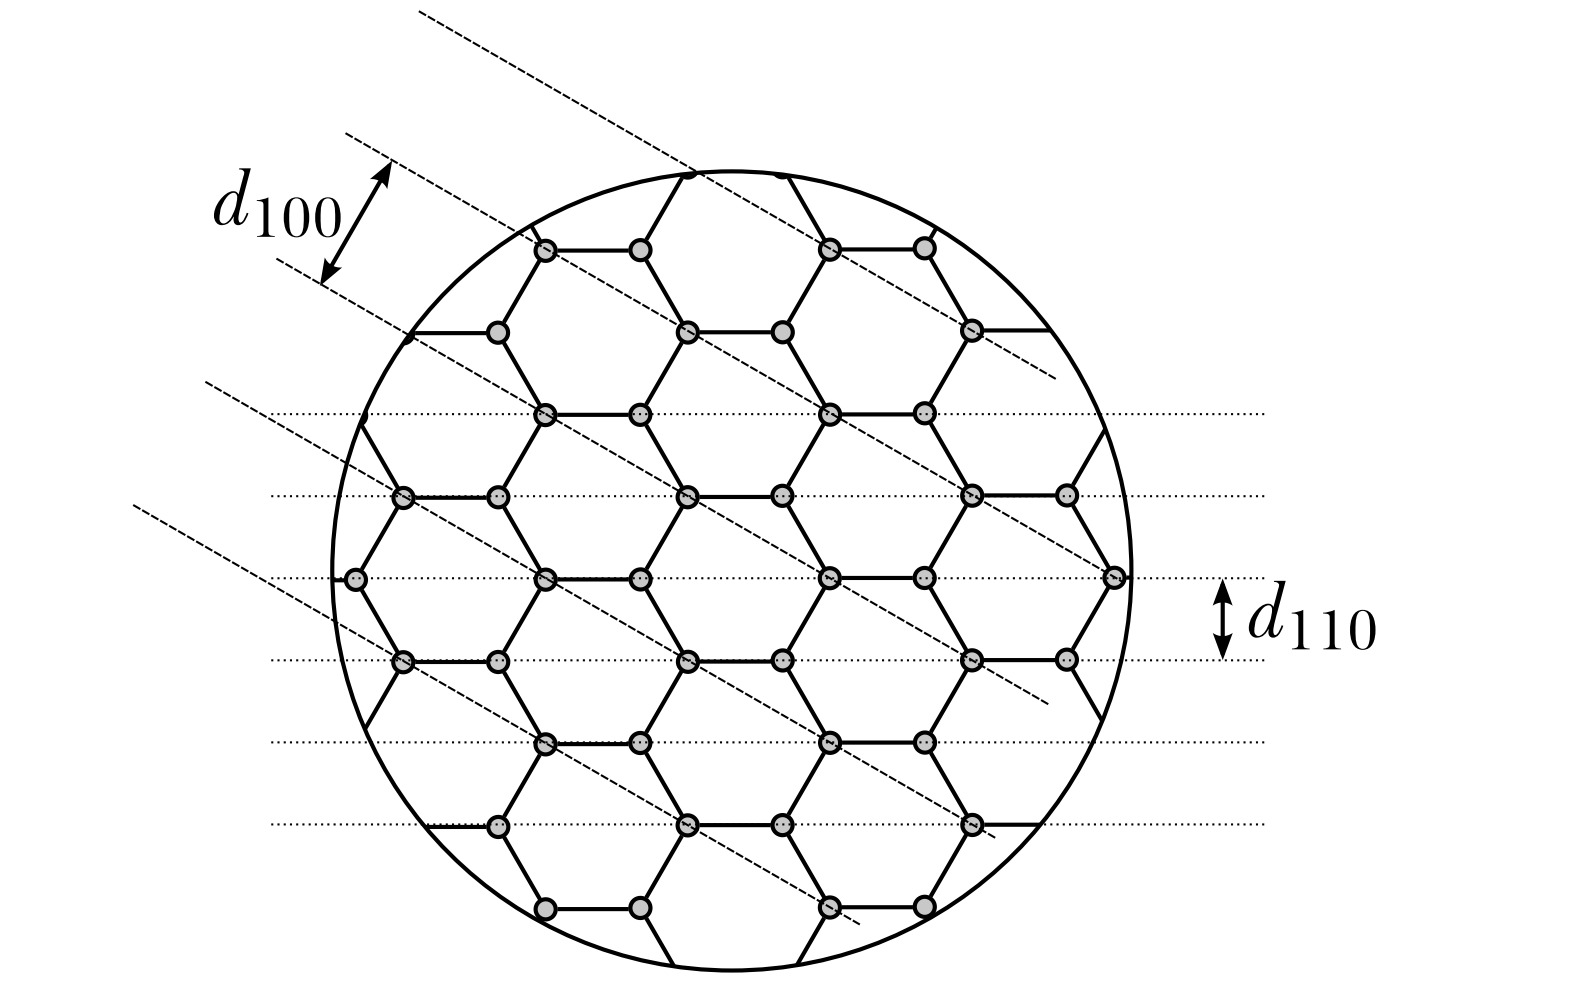
\includegraphics[width=3.4in, angle=0]{UnitCell.png}
    \caption{Visual of the graphite unit cell annotated with physical representations of the $d_{100}$ and $d_{110}$ spacings}
    \label{fig:unit}
\end{figure}

Looking at Fig. \ref{fig:unit}, the spacing of $d_{100}$ is shown to be physically larger than the spacing of $d_{110}$. This would imply that the inner ring value $1.7 \pm 0.1 \text{ Å} $ corresponds to $d_{100}$ as it is the larger of the two values, and vice versa for the outer ring value and $d_{110}$.  

The last and final question concerns whether the values calculated from this experiment agree with the commonly accepted values for $d_{100}$ and $d_{110}$. Other experiments find the value for $d_{100}$ to be roughly $2.1319 \text{ Å}$   and $d_{110}$ to be rough $1.2308  \text{ Å}$\cite{Howe2003}. Comparing results, the values for $d_{100}$ are relatively far from each other while the values of $d_{110}$ were much closer. The $d_{110}$ value obtained from other sources is actually contained within the estimated uncertainty of this experiment's $d_{110}$ value, while $d_{100}$ is not even close.

\section{Conclusion}

This experiment used an apparatus similar to that used in the Davisson-Germer experiment to revisit the idea of wave-particle duality in physical matter, leveraging it to perform basic analysis of the interplanar spacing of graphite. By combining Bragg's law with de Broglie, it was determined that $\sin\theta \propto E^{-1/2}$. When experimental results demonstrated trends consistent with that linear relationship, the data was used to calculate values for interplanar spacing. Of the two values  $d_{100}=1.7 \pm 0.1 \text{Å} $ and  $d_{110}= 1.4\pm 0.2\text{Å}$, only $d_{110}$ was close to widely accepted values of its interplanar spacing. In either case, the difference likely stems from measurement error during this experiment. Using manual measurement tools on a circular bulb with fuzzy reflections is not the most accurate way of going about this kind of analysis. Even with inaccurate values, this experiment was successful in its demonstration of de Broglie's theory and the wave-like nature of matter. 

\section*{Data Availability Statement}
A Jupyter notebook containing all the experimental data, data analysis, figure generation, and additional information on uncertainty analysis can be found in the supplemental materials. \footnote{See online article posting for access to supplemental material.}


% The \nocite command causes all entries in a bibliography to be printed out
% whether or not they are actually referenced in the text. This is appropriate
% for the sample file to show the different styles of references, but authors
% most likely will not want to use it.
%\nocite{*}

\bibliography{apssamp}% Produces the bibliography via BibTeX.

\end{document}
%
% ****** End of file apssamp.tex ******
